\chapter{Reinforcement Learning}
Here, the learner does not receive a labeled dataset, in contrast with supervised learning. Instead, he collects information through a course of actions by interacting with the environment. In response to an action, the learner or agent receives two types of information: his current state in the environment and a real-valued reward, which is specific to the task and its corresponding goal. Fig. \ref{fig:reinf_learn} shows the general scenario of reinforcement learning. Unlike supervised learning, there is no fixed distribution according to which the instances are drawn; the choice of a policy defines the distribution.

\begin{figure}[h]
\centering
\includegraphics[width=0.75\textwidth]{reinf_learn}
\caption[width=\textwidth]{\textbf{Representation of general scenario of Reinforcement learning}}
\label{fig:reinf_learn}
\end{figure}

The objective of the agent is to maximize his reward and thus to determine the best course of actions, or policy, to achieve the objective. \textbf{However, the information he receives from the environment is only the immediate reward corresponding to the action just taken. No future or long-term reward feedback is provided by the environment.} The agent also faces the dilemma between exploring unknown states and actions to gain more information about the environment and exploiting the information already collected to optimize his reward. Two main settings are possible:
\begin{enumerate}
    \item Environment model is known to agent. Then the problem is reduced to \textbf{planning}.
    \item Environment model is unknown to agent. Then, he faces \textbf{learning} problem. This will be our main concern.
\end{enumerate}

\section{Markov Decision Process Model}
A MDP is defined by:
\begin{enumerate}
    \item Set of states, $S$.
    \item Set of actions, $A$.
    \item Start state, $s_{0} \in S$.
    \item Reward Probability  
    \begin{equation} \label{eq:rew_prob}
    P(r_{t+1} | s_{t}, a_{t}) \hspace{0.2cm} where \hspace{0.1cm} r_{t+1} = r(s_{t}, a_{t})
    \end{equation}
    \item State transition probability
    \begin{equation} \label{eq:state_trans_prob}
    P(s_{t+1} | s_{t}, a_{t}) \hspace{0.2cm} where \hspace{0.1cm} s_{t+1} = \delta(s_{t}, a_{t})
    \end{equation}
\end{enumerate}

\begin{figure}[h]
\centering
\includegraphics[width=0.75\textwidth]{mdpm}
\caption[width=\textwidth]{Illustration of states and transitions of MDP at different times}
\label{fig:mdpm}
\end{figure}

We also define $\pi:S \rightarrow A$ as the policy function mapping a state S to an action A. In a discrete time model, actions are taken at a set of decision epochs $\left \{ 0, ..., T \right \}$. We deal with infinite horizon i.e. T tends to infinity. Now, the agent's objective is to find a policy that maximizes his expected reward.


\section{Policy Value}
We define the policy value  $V_{\pi}(s)$ in the case of infinite horizon as the expected reward of the agent starting at state $s$ and following policy $\pi$ i.e.
\begin{equation} \label{eq:polVal}
V_{\pi}(s) = E\bigg[ \sum_{\tau=0}^{T-t} \gamma^\tau r(s_{t+\tau}, \pi(s_{t+\tau})) | s_{t} = s \bigg]
\end{equation}
where $T$ tends to infinity.

The policy value  $V_{\pi}(s)$ obey the following system of linear equations (Bellman's equation):
\begin{equation} \label{eq:bellman}
\forall s \in S,\hspace{0.2cm} V_{\pi}(s) = E\big[ r(s,\pi(s))\big] + \gamma \sum_{s^{'}} Pr\bigg[s^{'}|s,\pi(s) \bigg] V_{\pi}(s^{'}) 
\end{equation}
Refer appendix for the proof.

The Bellman's equation can also be written as:
\begin{equation} \label{eq:bellman2}
\textbf{V} = \textbf{R} + \gamma \textbf{PV}
\end{equation}
where,\\ 
$\textbf{P}$ is the state transition probability matrix, 
$\textbf{R} = E[r(s,\pi(s))]$, 
$\gamma$ is the discount for future rewards and $\textbf{V}$ is the unknown policy value matrix

For a finite MDP, Bellman's equation admits a unique solution given by
\begin{equation} \label{eq:bellmanSol}
\textbf{V}_{0} = (\textbf{I}-\gamma \textbf{P})^{-1} \textbf{R} 
\end{equation}
Refer appendix for the proof.

The optimal policy value at a given state $s$ is thus given by 
\begin{equation} \label{eq:optPolVal}
V_{\pi^{*}}(s) = max_{\pi} V_{\pi}(s)
\end{equation}

\section{State-Action Value Function and Q-Learning}

We define the optimal state-action value function $Q^{*}$ for all $(s,a) \in S \times A$  as the expected return for taking action $a \in A$ at state $s \in S$ and then following the optimal policy:
\begin{equation} \label{eq:optimalPol}
Q^{*}(s,a) = E\big[ r(s,a) \big]  + \gamma \sum_{s^{'} \in S} Pr\big[  s^{'} | s, a \big]  V^{*}(s^{'}) 
\end{equation}
One can observe that the optimal policy can be given by
\begin{equation} \label{eq:optimalPolObs}
 \forall s \in S,\hspace{0.2cm} \pi^{*}(s) = argmax_{a \in A} Q^{*}(s,a) 
\end{equation}
Thus, the knowledge of the state-vale function $Q^{*}$ is sufficient for the agent to determine the optimal policy, without any direct knowledge of the reward or transition probabilities.

To learn the optimal state-action value function, Q-learning algorithm can be used as shown in Fig. \ref{fig:qlearning}

\begin{figure}
\centering
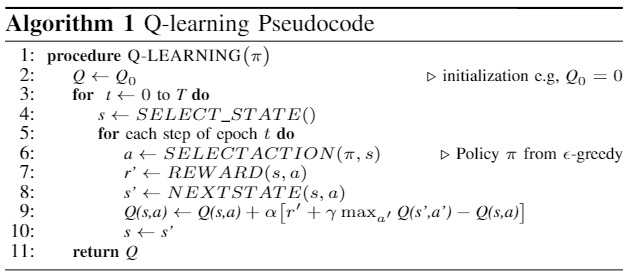
\includegraphics[width=0.75\textwidth]{qlearning}
\caption{\textbf{Q-Learning Algorithm}}
\label{fig:qlearning}
\end{figure}